\documentclass[a4paper,10pt]{article}
\usepackage{fontspec}
\defaultfontfeatures{Mapping=tex-text,Ligatures=TeX}
\usepackage[inner=3cm,top=3cm,outer=3cm,bottom=3cm]{geometry}
\usepackage[parfill]{parskip}
\usepackage{csquotes}
\usepackage{amsmath}
\usepackage{amssymb}
\usepackage{mathtools}
\usepackage{verbatim}
\usepackage{algpseudocode}
\usepackage{float}
\usepackage{tikz}
\usepackage{mathtools}
\usepackage[ireport]{pkg/KTHEEtitlepage}
\DeclarePairedDelimiter\ceil{\lceil}{\rceil}
\DeclarePairedDelimiter\floor{\lfloor}{\rfloor}
\usepackage[backend=biber]{biblatex}
\addbibresource{references/bibliography.bib}

\def\theauthor{Axel Riese \& André Nyström}
\def\thedate{\today}

\date{\thedate}
\author{\theauthor}

\def\assignment{Thesis}
\title{\assignment}

\begin{document}
% Information to appear on the title page:
\ititle{My Title}
\isubtitle{My Subtitle}
\iauthor{Me and Myself}
\idate{2006}
\irefnr{IR-EE-Dummy 2000:099}

\iaddress{Signal Processing\\
  School of Electrical Engineering\\
  Kungliga Tekniska Högskolan}
\makeititle

% Everything below is exactly as for a normal document and 
% the layout of that document should not be affected in any
% way by the title page.

\title{Short example of the KTHEEtitlepage package}
\author{Mats Bengtsson}

\maketitle

\section{Introduction}

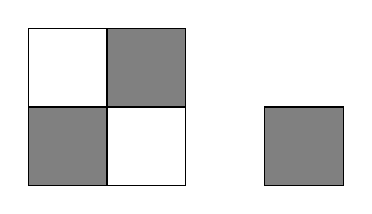
\begin{tikzpicture}
    \filldraw[fill=gray, draw=black] (0,0) rectangle (1,1);
    \filldraw[fill=white, draw=black] (1,0) rectangle (2,1);
    \filldraw[fill=white, draw=black] (0,1) rectangle (1,2);
    \filldraw[fill=gray, draw=black] (1,1) rectangle (2,2);

    \filldraw[fill=gray, draw=black] (3,0) rectangle (4,1);
    %\filldraw[fill=white, draw=black] (1,0) rectangle (2,1);
    %\filldraw[fill=white, draw=black] (0,1) rectangle (1,2);
    %\filldraw[fill=gray, draw=black] (1,1) rectangle (2,2);
\end{tikzpicture}

\input{thesis/objective.tex}
\section{Background}
\label{sec:background}

\subsection{Reduction}
A reduction is an algorithm used to solve one problem with another. This report consider only \textit{desicion problems}, which given some input must be either true (yes) or false (no).

A reduction from any decision problem $A$ to any other decision problem $B$ is valid if each yes-instance of $A$ yields a yes-instance of $B$, and each no-instance of $A$ yields a no instance of $B$. If the reduction runs in polynomial time, $B$ must be at least as hard as $A$ to solve.\cite{reduction}

\subsection{NP and PSPACE}
\textit{NP} is defined as the set of all decision problems where a yes-instance can be verified in polynomial time. If it is possible to reduce all problems in NP to a particular problem, that problem is defined to be \textit{NP-hard}. A problem is defined to be \textit{NP-complete} if it is both in NP and NP-hard. From this follows that if there exists a polynomial reduction from any NP-complete problem to some problem in NP, that problem is NP-complete as well. This is a commonly used method when proving NP-completeness for new decision problem.

PSPACE is the set of all decision problems that can be solved by a Turing machine in a polynomial amount of memory space. Similar to NP-complete, a problem is PSPACE-complete if it is in PSPACE and all other problems in PSPACE can be reduced to the problem.

\subsection{The Subset Sum problem}

The \textit{Subset Sum} Problem is defined as follows \cite[p.~491]{algorithm}:

\begin{quote}
Given natural numbers $w_1, \ldots, w_n$, and a target number $W$, is there a subset of $\{w_1, \ldots, w_n \}$ that adds up precisely to $W$?
\end{quote}

The Subset Sum Problem plays a crucial role in the proof presented later in this report. It is known to be NP-complete \cite[p.~492]{algorithm}. In fact it is a special case of the Knapsack Problem \cite[p.~491]{algorithm}, one of Karp's 21 NP-complete problems he discusses in his 1972 paper \cite{karp}.

\subsection{Previous studies}

In this section we will present some recent papers regarding computational complexity in video games.

\subsubsection{Classical Nintendo Games}

In one paper on Classical Nintendo Games, the computational complexity of games in the popular Nintendo series Legend of Zelda, Mario, Metroid, Donkey Kong and Pokémon are proven to be either NP- or PSPACE-hard \cite{classic}. The paper states that it is easy to understand that most games are members of PSPACE because their behaviour is a ``deterministic function of the player's controller input''. The paper focuses if it is possible to get from point A to point B on a generalized gameboard in these games. Using the NP-complete problem \textit{3-SAT} the authors build a framework of \textit{gadgets} to prove NP-hardness. For PSPACE-hardness a similar framework is used with the PSPACE-complete problem \textit{True Quantified Boolean Formula}. The framework gives the authors a simple way to show NP- and PSPACE-hardness by building the gadgets as gameboards in the respective games. The authors also use previous studies on the \textit{Push-1} \cite{push1} and \textit{PushPush-1} \cite{pushpushk} to show NP-hardness, respectively PSPACE-hardness, in some of the games implementing these problems as puzzles. 

\subsubsection{Lemmings}

Lemmings is a 2D puzzle-platformer game where the objective is to guide a couple of characters called lemmings through obstacles to reach a designated exit by giving the lemmings abilities such as digging or building. In one paper a proof that Lemmings is NP-complete is presented that uses gadgets. This is similiar to the proof of the classical Nintendo games. The authors of the paper also use the 3-SAT problem to prove NP-hardness. 

\subsubsection{Minesweeper}
Minesweeper is a popular puzzle game shipped with the Windows operating system. The game is played on a $n \times m$ gameboard where random cells are designated to contain mines. The goal of the game is to clear all cells except the ones containing the mines. In one paper on Minesweeper, the author use SAT to prove NP-hardness by building Minesweeper configurations of logic circuits consisting of NOT-, AND- and XOR-gates \cite{minesweeper}.

\subsubsection{Match-three games}

Candy Crush and Bejeweled are both popular puzzle games with the same concept of match-three. The games consists of grids where each cell contains one ``gem''. The player is allowed to swap a gems position in vertical and horizontal directions if she is able to match three gems of the same kind. When three gems of a kind is matched, the gems are ``popped'' and the gems above the now empty cells fall down to take their place. At the same time, the empty cells at the top are filled with new gems. In one paper the authors consider the offline version of Bejeweled and shows NP-hardness for general match-three games using the NP-complete \textit{1-in-3PSAT} problem \cite{candy}.

\subsubsection{Tetris}

Tetris is a popular puzzle game where the player is given a sequence of  four-sized blocks, ``tetrominoes'', to pack into a grid-based rectangular gameboard. If a row is completely filled it is cleared and all pieces above the cleared row is dropped by one row. In one paper the authors
shows the NP-completeness of offline Tetris wih specific goals using the NP-complete \textit{3-Partition} problem \cite{tetris}. Some considered goals are the number of cleared rows and for how long the player can survive. The reduction is done by building a Tetris gameboard from instances of the 3-Partition problem. A specific sequence of pieces are then defined for each number in the 3-Partition instance. In the same paper, it is also shown that Tetris is highly inapproximable. 

\subsection{Lumines and its similarities to Tetris}
\label{subsub:sim}

The existing research on Lumines largely focus on effective strategies. One paper states that there exists strategies that can never lose when starting on an empty gameboard, no matter what sequence of pieces are dropped \cite{lumines}. This is different to Tetris where losing can be inevitable if the computer is allowed to change the sequence according to how the player organizes the pieces \cite[p. 4]{tetris}. Another relevant difference brought up in prior research is that in Lumines it is possible to create terrain that can not be cleared, while in Tetris a gameboard can always be cleared if the player is given an appropriate sequence of pieces.

The standard Lumines game is played on a $10 \times 16$-gameboard, while standard Tetris is played on a $20 \times 10$-gameboard. In both games, when any block is fixed outside of the gameboard the player loses the game. The player is also given the same kind of control of the pieces i.e. rotating, horizontal movement and dropping the piece.

While in Tetris a completed row is removed instantly, the marked cells in Lumines is not removed until the sweep-line has scanned the area. This creates interesting strategies with timing which does not exist in Tetris. Waiting before dropping a piece in Tetris does not give the player an advantage more than the time to think about what to do next. In Lumines however a player can wait for the sweep-line to scan terrain before dropping a block that would otherwise be cleared for the possibility of clearing more terrain when the sweep-line scans again.

The fact that falling blocks may seperate after being fixed in Lumines implies that there aren't as many ways to build unique terrain as in Tetris. Nevertheless some significant similarities exist between the two games, making the existing research on Tetris a valuable asset when considering the complexity of Lumines.

\section{Method}
\subsection{Finding a reduction}
As mentioned in \ref{subsub:sim} there exists many similarities between Lumines and the more thoroughly researched video game Tetris. This fact suggested that is was a good idea to draw inspiration from papers concerning the computational complexity of Tetris. In one such paper by \citeauthor{tetris}, the authors present a reduction from \textit{3-Partition} to the problem of how many rows can be cleared using some sequence of Tetris pieces (for more information see \cite{tetris}). Although we considered a proof of similar completeness to be out of the scope of this report, we were inspired by the notion of forcing game pieces to be placed in certain positions by creating a precise initial gameboard and limiting the sequence of game pieces to fewer kinds. The forced placement of a game pieces in turn forces the placement of the next game piece and so on. In the case of the reduction found in the Tetris paper, the height of this predetermined stack of game pieces determines how many rows of the gameboard that can be cleared.

When looking for a suitable problem to reduce to our problem, we focused on the NP-hard problems we had priorly encountered in literature and courses. We then examined whether a problem would fit nicely in this characteristic of forced placement and game piece stacking. We finally decided to turn our attention to the \textit{Subset sum} problem, which was both fairly well understood by us and seemed to have a simple mapping from some parts of a problem instance to some parts of our problem instances. For example it seemed plausible that a set elements $n$ in a \textit{Subset sum} instance could be mapped to $n$ Lumines blocks of the same kind in a sequence, and the additive characteristic of elements in a \textit{Subset sum} instance seemed like a good match for the stacking characteristic of Lumines gameplay.
\input{thesis/results.tex}
\section{Discussion}
\label{discussion}

\subsection{Rotations}

The two main ways the player can control the Lumines game found on the PSP is to rotate and move the blocks left and right. A simplified model where the player is not allowed to rotate the blocks has been used in the reduction given in this report, meaning an important part of the game is not considered in the proof. It was planned to find a reduction which included rotations but because of time constraints this was not executed and a model without rotations was used instead. Intuitively rotation should have some impact on the hardness of the game. Because of the fact we found it harder to find a proper reduction of the Subset sum when a rotation model was used the possibility that Lumines is actually easier than NP-hard exist. However this does not have to be the case, rotations may as well be harder if it could be proven that an algorithm have to consider all possible ways to build terrain. During this project nothing has been found that tells us how rotations change the complexity and should therefore be examined to get a better understanding of the real game's complexity.

\subsection{Sweep-line}

In Lumines the sweep-line moves in constant speed from left to right. The marked squares are then cleared as the sweep-line scans the cells in their respective marked squares. The simplified Lumines model that is presented in this paper uses an instant sweep-line, in which the cells are marked and cleared simultaneously when a square is formed. This is similar to how rows are cleared in Tetris, but not the most accurate representation of how the sweep-line works in Lumines. There is probably room for improvement in making a more accurate model of the sweep-line game mechanic. For example, every $n\text{th}$ block that is fixed could trigger the clearing of marked cells. The less accurate model in this report was chosen since it was more suitable to work with given the time limit of the project. It is however important to note that the amount of cells that can be cleared in a given sequence can vary dramatically between different models of the sweep-line (see \textbf{todo figure showing this}). Therefore, in future work, inquires into the impact of the chosen sweep-line model on the computational complexity would be a promising area of research.

\subsection{Online Lumines}

In the reduction and proof of Lumines complexity presented in this paper the offline version of Lumines has been considered. This is similar to previous studies on Match-three games and Tetris. In these reports they argue that if a property can be shown in the offline version of the games intuitively it should not be easier in the online version. According to Demaine, Hoffman and Holzer, ``...it is only easier to play Tetris with complete knowledge of the future, so the difficulty of playing the offline version suggests the difficulty of playing the online version'' \cite[p. 2]{tetris}. If this is true it should also be the case for Lumines. However none of the papers that has been examined present any proof that this is the case. Therefore the online version of Lumines should be examined in the future to research if any such proof can be conducted.

\subsection{Subset sum}

During the research before our reduction was conducted, none of the reductions examined used the subset sum. The most common problem to reduce from seems to be 3-SAT. It is the author's beliefs that this is the first instance concerning video game complexity using the subset sum problem. The nature of NP-completeness permits any NP-complete problem to be used in principle but some problems are inherently easier to reduce than others. The results from this report shows that the subset sum problem is suitable for use when reducing to 2D stacking grid games similar to Lumines. 

\printbibliography
\end{document}
